\section*{Multiple-choice}\label{sec:mc}

Dine svar skal indtastes i ITX-systemets multiple-choice modul.

\multiplechoicestart

\spoergsmaal{Rekursionsligninger}
Hvilke af følgende rekursionsligninger, med antagelsen at $T(n)=1$ for $n\leq 1$, har løsningen $T(n)=\Theta(n \log n)$? \fleresvar
\mulighederstart
\svar $T_1(n) = 3\cdot T_1(n/3) + \Theta(n)$ \korrekt
\svar $T_2(n) = T_2(n/2) + \Theta(n \log n)$ \korrekt
\svar $T_3(n) = 3\cdot T_3(n/4) + \Theta(n)$
\svar $T_4(n) = 2\cdot T_4(n/2) + \Theta(1)$
\svar $T_5(n) = 4\cdot T_5(n/2) + \Theta(n)$
\svar $T_6(n) = T_6(n-1) + \Theta(\log n)$ \korrekt
\mulighederslut
\forklaring{Ligning $T_1$ løses med master theorem til $\Theta(n \log n)$, og for $T_2$ med $a=1$, $b=2$ og $f(n)=\Theta(n \log n)$ opnås samme vækstrate. De øvrige rekursioner har andre løsninger, der kan findes med master theorem.}

\spoergsmaal{Rekursive algoritmer}
En rekursiv algoritme \(A\) virker således på input \(x\) af størrelse \(n\):
\begin{itemize}
  \item Hvis \(n=1\), returneres et svar i tid \(\Theta(1)\).
  \item Ellers:
  \begin{itemize}
    \item Der bruges tid \(\Theta(n)\) på at beregne to delresultater \(x_1\) og \(x_2\), hver af størrelse \(n-1\).
    \item Algoritmen kaldes rekursivt på \(x_1\) og \(x_2\), hvorefter svarene \(y_1\) og \(y_2\) modtages.
    \item Svarene \(y_1\) og \(y_2\) kombineres til et svar i tid \(\Theta(1)\).
  \end{itemize}
\end{itemize}
Hvilken rekursionsligning beskriver bedst køretiden \(T(n)\) for algoritmen \(A\) med basistilfældet \(T(1)=1\)?
\etsvar
\mulighederstart
\svar \(T(n)=2\,T(n/2)+\Theta(1)\)
\svar \(T(n)=2\,T(n/2)+\Theta(n)\)
\svar \(T(n)=2\,T(n/2)+\Theta(2^n)\)
\svar \(T(n)=2\,T(n-1)+\Theta(1)\)
\svar \(T(n)=2\,T(n-1)+\Theta(n)\) \korrekt
\svar \(T(n)=2\,T(n-1)+\Theta(2^n)\)
\mulighederslut
\forklaring{Der udføres to rekursive kald på input af størrelse \(n-1\), og derudover bruges $\Theta(n)$ tid på at beregne de to delresultater og $\Theta(1)$ tid på at kombinere dem, hvilket samlet giver $\Theta(n)$. Dermed får vi rekursionsligningen \(T(n)=2T(n-1)+\Theta(n)\).}

\spoergsmaal{Invarianter}
Betragt denne algoritme, der tager et array $A[1:n]$ af heltal samt et heltal $k$ som input.
\begin{codebox}
\Procname{$\proc{Two-Sum-BruteForce}(A, n, k)$}
\li \For $i \gets 1$ \To $n-1$
\li \Do
        \For $j \gets i+1$ \To $n$
\li     \Do
            \If $A[i] + A[j] = k$
\li         \Then \Return \const{True}
         \End
        \End
    \End
\li \Return \const{False}
\end{codebox}
Hvilke af følgende invarianter gælder (for ethvert input) i \emph{begyndelsen} af hver iteration af den ydre løkke? 
I hver iteration har variablen $i$ værdierne $1, 2, \dots$ og invarianten evalueres med hensyn til den aktuelle værdi af $i$ under den givne iteration.
Invarianten skal ikke nødvendigvis gælde, hvis linje 4 udføres, og iterationen derfor afbrydes.
\fleresvar
\mulighederstart
\svar For alle $i',j'$ med $1\leq i' < i$ og $1\leq j'<i$ er $A[i']+A[j'] = k$
\svar For alle $i',j'$ med $1\leq i' < i$ og $1\leq j'<i$ er $A[i']+A[j'] \ne k$
\svar For alle $i',j'$ med $1\leq i' < i$ og $j'\in\{1,\dots,n\}\backslash\{i'\}$ er $A[i']+A[j'] = k$
\svar For alle $i',j'$ med $1\leq i' < i$ og $j'\in\{1,\dots,n\}\backslash\{i'\}$ er $A[i']+A[j'] \ne k$ \korrekt
\mulighederslut
\forklaring{I iteration $i$ undersøges det, om der findes noget $j$, således at $A[i]+A[j]=k$. Par af indekser der allerede er undersøgt springes over ved at starte den indre løkke med $j=i+1$. Derfor er invariant 4 sand. Invariant 1 og 3 fejler efter højst to iterationer hvis fx $A = \langle 0, 0, 0\rangle$ og $k=1$. Invariant 2 fejler hvis der findes $j'$ hvor $A[j'] = k/2$, da vi i tilfældet $i'=j'$ så har $A[i']+A[j'] = k$.}

\spoergsmaal{Enigma}
Betragt denne algoritme, der som input tager et array $A[1:n]$ og to indekser $i,j$ med $i\leq j$, og som ændrer på arrayet $A$.
\begin{codebox}
  \Procname{$\proc{Enigma}(A, i, j)$}
  \li \If $j\leq i+1$ \textbf{ and } $A[j]<A[i]$ \Do
  \li swap $A[i]$ with $A[j]$  \li \ElseIf $j>i+1$ \Do
  \li $\proc{Enigma}(A,i,j-1)$
  \li $\proc{Enigma}(A,i+1,j)$
  \li $\proc{Enigma}(A,i,j-1)$
  \End
\end{codebox}
Hvilke af følgende udsagn gælder når vi kalder $\proc{Enigma}(A, 1, n)$?
%, hvor $A$ er et array af længde~$n$?
\fleresvar
\mulighederstart
\svar Algoritmen danner alle permutationer af tallene i $A$ før den terminerer.
\svar Algoritmen sorterer $A$ ikke-aftagende orden.\korrekt
\svar Algoritmen sorterer $A$ i ikke-stigende orden.
\svar Køretiden er $\Theta(n \log n)$.
\svar Køretiden er $\Theta(n^3)$.
\svar Køretiden er $\Theta(3^n)$.\korrekt
\svar Køretiden er $\Theta(n!)$.
\mulighederslut
\forklaring{Algoritmen sorterer $A$ i ikke-aftagende orden, hvilket kan ses ved et induktionsbevis. Efter de to første rekursive kald er det maksimale element på den sidste plads. Derfor rækker det sidste rekursive kald til at færdiggøre sorteringen. Tiden overholder rekursionsformlen $T(n) = 3 T(n-1) + O(1)$, der kan løses ved substitutionsmetoden til $\Theta(3^n)$ tid.}

\spoergsmaal{Arbejde og spand}
Betragt denne parallelle algoritme, der tæller antal knuder i et binært træ, givet ved sin rodknude $T$.
En knude $T$ har børn $T.left$ og $T.right$, hvor værdien $\proc{nil}$ bruges til at indikere det tomme træ.

\begin{codebox}
\Procname{$\proc{Parallel-InOrder-Count}(T)$}
\li \If $T = \proc{nil}$ 
\li \Then \Return $0$
\li \Else
%\li     $leftCount \gets 0$
%\li     $rightCount \gets 0$
\li     \Spawn $leftCount \gets \proc{Parallel-InOrder-Count}(T.\id{left})$
\li     $rightCount \gets \proc{Parallel-InOrder-Count}(T.\id{right})$
\li     \Sync
\li     \Return $leftCount + rightCount + 1$
\end{codebox}
Hvis træet med rodknude $T$ har $n$ knuder og højde $h$, hvad er algoritmens arbejde (eng.~\emph{work}) og spand (eng.~\emph{span})?
\etsvar
\mulighederstart
\svar Arbejde $T_1=\Theta(n)$, spand $T_\infty=\Theta(\log h)$
\svar Arbejde $T_1=\Theta(n)$, spand $T_\infty=\Theta(\log n)$
\svar Arbejde $T_1=\Theta(n)$, spand $T_\infty=\Theta(h)$ \korrekt
\svar Arbejde $T_1=\Theta(h)$, spand $T_\infty=\Theta(\log h)$
\svar Arbejde $T_1=\Theta(h)$, spand $T_\infty=\Theta(\log n)$
\svar Arbejde $T_1=\Theta(h)$, spand $T_\infty=\Theta(h)$
\mulighederslut
\forklaring{De rekursive kald udføres parallelt og alt andet tager konstant tid. Derfor er algoritmens spand proportional med rekursionsdybden $h$. Arbejdet er proportionalt med antal knuder da algoritmen bruger konstant tid på hver knude.}

\spoergsmaal{Parallelle algoritmer}
Antag at en parallel algoritme på input af størrelse $n$ har arbejde (eng.~\emph{work}) $T_1=\Theta(n \log n)$ og spand (eng.~\emph{span}) $T_\infty=\Theta(n)$.
Vi er interesserede i tiden $T_P$ der bruges til at køre algoritmen på $P$ processorer med grådig opgaveplanlægning (eng.~\emph{greedy scheduling}).
Hvilke af nedenstående påstande er korrekte?
\fleresvar
\mulighederstart
\svar Hvis $P = \Theta(1)$ så er $T_P = O(n^2)$ \korrekt
\svar Hvis $P = \Theta(\log{n})$ så er $T_P = O(n)$ \korrekt
\svar Hvis $P = \Theta(\sqrt{n})$ så er $T_P = O(\sqrt{n})$
\svar Hvis $P = \Theta(n)$ så er $T_P = O(\log n)$
\svar Hvis $P = \Theta(n \log n)$ så er $T_P = O(1)$
\mulighederslut
\forklaring{Ifølge CLRS Theorem 26.1 er $T_P \leq T_1 / P + T_\infty$, og denne grænse er ifølge Theorem 26.2 indenfor en faktor 2 den sande køretid. Ved at indsætte værdierne af $P$ får vi følgende grænser: 1. $T_P = \Theta(n \log n + n) = \Theta(n \log n)$, 2. $T_P = \Theta(n \log(n)/\log n + n) = \Theta(n)$, 3. $T_P = \Theta(n \log(n)/\sqrt{n} + n) = \Theta(n)$, 4. $T_P = \Theta(n \log(n) / n + n) = \Theta(n)$, 5. $T_P = \Theta(n \log(n) / (n \log n) + n) = \Theta(n)$. Dette medfører grænsen 1. og matcher grænsen 2., men er dårligere end grænserne i 3., 4. og 5.
}

\sideskift

\spoergsmaal{Invarianter for dynamiske tabeller}
Betragt dynamiske tabeller som beskrevet i CLRS sektion 16.4.2, altså versionen med en {\sc Table-Delete} operation.
Hvilke af følgende udsagn udgør gyldige invarianter, der gælder efter hver {\sc Table-Insert} og {\sc Table-Delete} operation?
Bemærk at de mulige invarianter ikke er uafhængige, vi har at $1 \Rightarrow 2 \Rightarrow 3$ og $4 \Rightarrow 5 \Rightarrow 6$.
\fleresvar
\mulighederstart
\svar $T.size \leq T.num$
\svar $T.size \leq 2\cdot T.num$
\svar $T.size \leq 4\cdot T.num$ \korrekt
\svar $T.num \leq T.size$ \korrekt
\svar $T.num \leq 2\cdot T.size$ \korrekt
\svar $T.num \leq 4\cdot T.size$ \korrekt
\mulighederslut
\forklaring{Operationerne er implementeret således at antal elementer $T.num$ kan variere mellem 25\% og 100\% af tabellens kapacitet, $T.size$.
Svarmulighed 5 og 6 giver løse øvre grænser, men er ikke desto mindre gyldige invarianter.}

\spoergsmaal{Tidskompleksitet for Fibonaccihobe}
Antag, at der udføres en {\sc Fib-Heap-Decrease-Key} operation på en Fibonaccihob $H$ med $n$ nøgler, som beskrevet i CLRS digitalt kapitel 19.
Det faktiske tidsforbrug for operationen er ikke nødvendigvis identisk med det amortiserede tidsforbrug.
Lad potentialfunktionen før operationen have værdien $\Phi(H)$ og efter operationen $\Phi(H')$.
Hvad kan vi med sikkerhed sige om det faktiske tidsforbrug af denne ene {\sc Fib-Heap-Decrease-Key} operation?
\fleresvar
\mulighederstart
\svar Tiden er $O(1)$
\svar Tiden er $O(\log n)$
\svar Tiden er $O(n)$ \korrekt
\svar Tiden er $O(1 + \Phi(H') - \Phi(H))$
\svar Tiden er $O(1 + \Phi(H) - \Phi(H'))$ \korrekt
\mulighederslut
\forklaring{Den amortiserede analyse af {\sc Fib-Heap-Decrease-Key} viser, at operationen kører i amortiseret $O(1)$ tid, hvor den præcise tidsbrug kan udtrykkes som $O(1 + \Phi(H) - \Phi(H'))$.
Køretiden er begrænset af antal ``cascading cuts'' som er $O(n)$ men ikke nødvendigvis $O(1)$ eller $O(\log n)$.
Værdien $\Phi(H') - \Phi(H)$ kan være et negativt tal af størrelse $\Omega(n)$, så valgmulighed 4 er ikke korrekt.
}

\spoergsmaal{Stavudskæring}
Betragt algoritmen \textsc{Extended-Bottom-Up-Cut-Rod} som beskrevet i CLRS sektion 14.1.
På et ukendt input returnerer algoritmen en vektor $r$ med værdier og en vektor $s$ med stavlængder:
\[
r=\langle 0, 3, 6, 10, 13, 16, 20, 23, 26\rangle
\]
\[
s=\langle 1, 1, 3, 1, 1, 3, 1, 1 \rangle
\]
Hvor mange stænger (eng.~\emph{rods}) er der i den optimale løsning som kan beregnes ud fra $r$ og $s$?
\etsvar
\mulighederstart
\svar 2 stænger
\svar 3 stænger
\svar 4 stænger \korrekt
\svar 10 stænger
\svar 16 stænger
\svar 26 stænger
\mulighederslut
\forklaring{Længderne fremgår af $s$. $s[8]$ siger at vi skal starte med en stang af længde 1, indgang $s[7]$ siger at den næste stang også har længde 1, indgang $s[6]$ siger at den næste stang har længde 3, og indgang $s[3]$ siger at den sidste stang har længde 3. Dvs.~fire stænger totalt.}

\spoergsmaal{Længste fælles delsekvens}
Vi betragter algoritmen til længste fælles delsekvens (eng.~\emph{longest common subsequence}) i CLRS sektion 14.4 kørt på strengene SMOOTH og MOTOR.
Hvad skal indholdet være i de to felter markeret med {\bf X} og {\bf Y}?

\begin{center}
\begin{tabular}{c|c|c|c|c|c|c|c||}
    &   & S & M & O & O & T & H\\
    \hline
     & 0 & 0 & 0 & 0 & 0 & 0 & 0\\
     \hline
    M & 0 & $\uparrow0$ & $\nwarrow1$ & $\leftarrow1$ & $\leftarrow1$ & $\leftarrow1$ & $\leftarrow1$ \\
    O & 0 & $\uparrow0$ & $\uparrow1$ & $\nwarrow2$ & $\nwarrow2$ & $\leftarrow2$ & $\leftarrow2$ \\
    T & 0 & $\uparrow0$ & $\uparrow1$ & $\uparrow2$ & $\uparrow2$ & $\nwarrow3$ & $\leftarrow3$ \\
    O & 0 & $\uparrow0$ & $\uparrow1$ & {\bf X} & $\nwarrow3$ & $\uparrow3$ & $\uparrow3$ \\
    R & 0 & $\uparrow0$ & $\uparrow1$ & $\uparrow2$ & $\uparrow3$ & $\uparrow3$ & {\bf Y} \\
    \hline
\end{tabular}
\end{center}

\etsvar
\mulighederstart
\svar $X = \leftarrow2$, $Y = \uparrow3$
\svar $X = \nwarrow2$, $Y = \uparrow4$
\svar $X = \nwarrow2$, $Y = \uparrow3$ \korrekt
\svar $X = \leftarrow2$, $Y = \uparrow4$
\mulighederslut
\forklaring{Håndkørsel af algoritmen giver det markerede svar.}

\spoergsmaal{Huffman koder}
Betragt alfabetet \(C=\{a,b,c,d,e\}\) med frekvenserne
\[
f_a=40,\quad f_b=30,\quad f_c=20,\quad f_d=5,\quad f_e=4.
\]
Når Huffmans algoritme køres (jf.~CLRS afsnit 15.3), hvad er længden af det \emph{korteste} kodeord i den konstruerede kode?
\etsvar
\mulighederstart
\svar Længde 1\korrekt
\svar Længde 2
\svar Længde 3
\svar Længde 4
\mulighederslut
\forklaring{Algoritmen beregner dette træ (tegnet uden 0-1 labels på kanterne), hvor $a$ har et kodeord af længde 1 svarende til en sti af længde 1 fra roden:\medskip
\begin{center}
    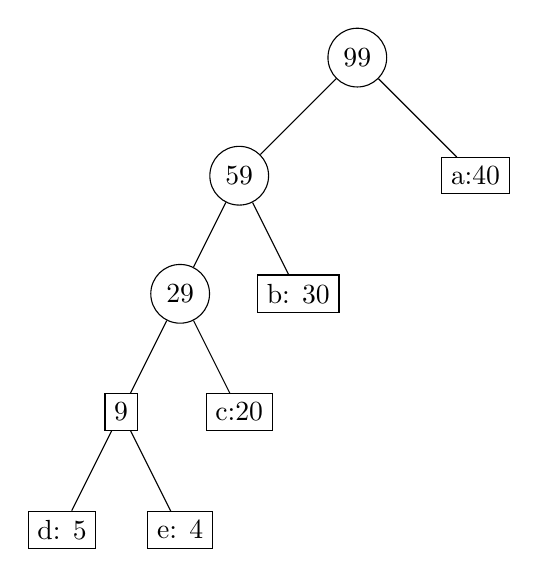
\begin{tikzpicture}[level distance=1.5cm,  level 1/.style={sibling distance=3cm},  level 2/.style={sibling distance=1.5cm}]
        \node [circle, draw] {99}
          child {node [circle, draw] {59}
            child {node [circle, draw] {29}
              child {node [rectangle, draw] {9}
                child {node [rectangle, draw] {d: 5}}
                child {node [rectangle, draw] {e: 4}}
              }
              child {node [rectangle, draw] {c:20}}
            }
            child {node [rectangle, draw] {b: 30}}
          }
          child {node [rectangle, draw] {a:40}
          };
      \end{tikzpicture}
\end{center}
}

\sideskift

\spoergsmaal{Matrixkæde-multiplikation}
Algoritmen {\sc Matrix-Chain-Order}$(p,n)$ fra CLRS 14.2 returnerer to arrays $m$ og $s$.
%Vi minder om at tabellen $s$ angiver hvordan man skal sætte parenteser i et produkt af matricer $A_1A_2\cdots A_n$ så det kan udregnes med færrest multiplikationer.
%Hvis $s[i,j]=k$ betyder det at de yderste parenteser i produktet $A_i\cdots A_j$ skal sættes som $(A_i\cdots A_k)(A_{k+1}\cdots A_j)$.
%
Nedenfor ses et array $s[1:n-1, 2:n]$ returneret af {\sc Matrix-Chain-Order}$(p,n)$ for et produkt af $n=6$ matricer $A_1\cdots A_6$ med dimensioner angivet i $p$.
\medskip

\begin{tabular}{c|cccccc}
$i \backslash j$ & 2 & 3 & 4 & 5 & 6 \\
\hline
1 & 1 & 1 & 1 & 1 & 1 \\
2 & & 2 & 2 & 4 & 4 \\
3 &     & & 3 & 4 & 4 \\
4 &     &     & & 5 & 5 \\
5 &     &     &     & & 5 \\
\end{tabular}

\medskip\noindent
Angiv måden at sætte parenteser på ifølge tabellen.
\etsvar
%
\mulighederstart
\svar $((A_1(A_2 A_3))((A_4 A_5)A_6))$

\svar $(A_1((A_2(A_3A_4))(A_5 A_6)))$ \korrekt

\svar $(((((A_1 A_2)A_3)A_4)A_5)A_6)$.

\svar $((((A_1 A_2)A_3)A_4)(A_5A_6))$.

\svar $((A_1(A_2 A_3))(A_4(A_5 A_6)))$
\mulighederslut
\forklaring{Håndkørsel af algoritmen {\sc Print-Optimal-Parens}$(s,1,n)$ giver det markerede svar.}

\spoergsmaal{Paradigmer}
Betragt følgende pseudokode, der tager et array $A$ og to indekser $p$, $r$ som parametre.
\begin{codebox}
  \Procname{$\proc{MyRecursiveAlgorithm}(A, p, r)$}
  \li \If $p<r$ \Do
  \li $q = \lfloor (p+r)/2\rfloor$
  \li \If $A[p]>A[q]$ \Do
  \li \Return 0
  \li \Else
  \li $x = \proc{MyRecursiveAlgorithm}(A, p, q)$
  \li $y = \proc{MyRecursiveAlgorithm}(A, q+1, r)$
  \li \Return $\min(x,y)$ \End
  \li \Else
  \li \Return 1\End
\end{codebox}
Hvilket af nedenstående paradigmer beskriver bedst $\proc{MyRecursiveAlgorithm}$?
\etsvar
\mulighederstart
\svar Del og hersk (eng.~\emph{divide and conquer}) \korrekt
\svar Dynamisk programmering (eng.~\emph{dynamic programming})
\svar Grådige algoritmer (eng.~\emph{greedy algorithms})
\mulighederslut
\forklaring{Algoritmen deler problemet op i to mindre dele, løser dem rekursivt og kombinerer resultaterne, hvilket kendetegner del og hersk paradigmet.}

\spoergsmaal{Rotationer i rød-sorte søgetræer}
Betragt dette rød-sorte søgetræ $T$, hvor bladene er udeladt:
\begin{center}
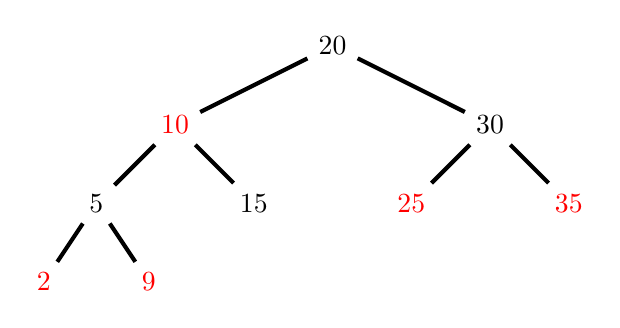
\begin{tikzpicture}[-,>=stealth,level/.style={sibling distance = 4cm/#1,
    level distance = 1cm}, line width=1.5pt] 
  \node [black] {20}
      child{ node [red] {10} 
              child{ node [black] {5} 
                    child{ node [red] {2} }
                    child{ node [red] {9} }
              }
              child{ node [black] {15} }                            
      }
      child{ node [black] {30}
              child{ node [red] {25} }
              child{ node [red] {35} }
          }
  ; 
  \end{tikzpicture}  
\end{center}

\noindent
Antag at vi kører algoritmen {\sc Right-Rotate$(T,10)$} (jf.~CLRS kapitel 13.2) med knuden $10$ som input. Hvad sker der med træet $T$?
\fleresvar
\mulighederstart
\svar 9 bliver venstre barn til 10 \korrekt
\svar 10 bliver højre barn til 5 \korrekt
\svar Højden af træet stiger med 1
\svar Højden af træet forbliver uændret \korrekt
\mulighederslut
\forklaring{Efter en højre rotation med knuden $10$ flyttes knuden $5$ op, og $10$ bliver dens højre barn. Træets højde forbliver den samme da 10's undertræ er lavere end 5's undertræer.}

\spoergsmaal{Korteste veje}
I denne opgave er vi interesserede i korteste veje på en graf med $n$ knuder, hvor hver knude har en kant til $d$ andre knuder, hvor $2\leq d < n$.
Til hver kant er knyttet en ikke-negativ vægt.
Vi ønsker at bruge Dijkstra's algoritme til at finde korteste veje fra en startknude $s$ til alle knuder i grafen.
Antag at algoritmen implementeres med en Fibonacci heap som prioritetskø.
Hvad kan vi sige om den asymptotiske køretid som funktion af $n$ og $d$?
\fleresvar

\mulighederstart
\svar Tiden er $O(nd + n \log d)$
\svar Tiden er $O(nd + n \log n)$ \korrekt
\svar Tiden er $O(nd + d \log d)$
\svar Tiden er $O(nd \log d)$
\svar Tiden er $O(n^2)$\korrekt
\svar Tiden er $O(n^2 \log d)$ \korrekt
\mulighederslut
\forklaring{ Tiden for Dijkstra's algoritme implementeret med Fibonacci heaps er $O(n \log(n) + m)$, hvor $m$ er antal kanter.
I den beskrevne situation er $m=dn$, hvilket giver at køretiden er $O(nd + n \log n)$.
Da $d < n$ medfører det at grænsen $O(n^2)$ er gyldig, og da $\log d \geq \log 2 > 0$ er grænsen $O(n^2 \log d)$ også gyldig.
Hvis $d=O(1)$ er de tre andre grænser $O(nd)$, lineært i antal kanter, hvilket er hurtigere end Dijkstra's algoritme der på værstefalds grafer med $O(n)$ kanter kører i tid $\Theta(n \log n)$.
}

\sideskift

\spoergsmaal{Mindste udspændende træ}
Betragt mindste udspændende træ-problemet på nedenstående graf:
\begin{center}
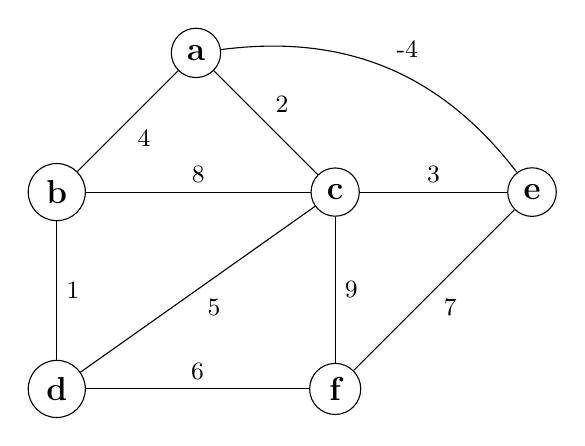
\begin{tikzpicture}[node distance=2.5cm, auto,>=stealth,
  main node/.style={circle,draw,font=\large\bfseries}]
  \node[main node] (a) {a};
  \node[main node] (b) [below left of=a] {b};
  \node[main node] (c) [below right of=a] {c};
  \node[main node] (d) [below of=b] {d};
  \node[main node] (e) [right of=c] {e};
  \node[main node] (f) [below of=c] {f};
  
  \path[every node/.style={font=\small}]
    (a) edge node {2} (c)
    (a) edge node {4} (b)
    (a) edge[bend left=30] node {-4} (e)
    (b) edge node {1} (d)
    (c) edge node {3} (e)
    (c) edge node {9} (f)
    (d) edge node {6} (f)
    (e) edge node {7} (f)
    (c) edge node {5} (d)
    (b) edge node {8} (c);
\end{tikzpicture}
\end{center}
Hvilke kanter indgår i det unikke mindste udspændende træ (MST)?
\fleresvar
\mulighederstart
\svar \{a,b\} \korrekt
\svar \{a,c\} \korrekt
\svar \{a,e\} \korrekt
\svar \{b,c\}
\svar \{b,d\} \korrekt
\svar \{c,d\}
\svar \{c,e\}
\svar \{c,f\}
\svar \{d,f\} \korrekt
\svar \{e,f\}
\mulighederslut
\forklaring{Ved at køre Kruskals algoritme vælges kanterne i stigende rækkefølge: \(\{a,e\}\) (vægt -4), \(\{b,d\}\) (vægt 1), \(\{a,c\}\) (vægt 2), \(\{a,b\}\) (vægt 4 ) og \(\{d,f\}\) (vægt 6). De øvrige kanter ville skabe en cykel. Prim's algoritme giver samme svar da kantvægtene er unikke.}

\spoergsmaal{Grafalgoritmer}
Antag at du har en uorienteret, vægtet graf med kantvægte mellem $-100$ og $+100$. 
Antallet af knuder er $n$ og antallet af kanter er $\binom{n}{2}$, dvs.~alle par af knuder er forbundet af en kant med vægt mellem $-100$ og $100$.
Hvilken af nedenstående algoritmer fra CLRS er det bedste valg til at beregne et mindste udspændende træ (MST)?
\etsvar
\mulighederstart
\svar Bredde-først søgning
\svar Bellman-Ford algoritmen
\svar Dijkstra's algoritme 
\svar Kruskal's algoritme \korrekt
\mulighederslut

\forklaring{Blandt de nævnte algoritmer er der kun én, nemlig Kruskal's algoritme, der returnerer et mindste udspændende træ. De andre returnerer \emph{korteste-veje træer} for forskellige typer af vægtede, orienterede grafer. Det har ingen betydning at vægtene kan være negative, eller at grafen er komplet.
%, men vi bemærker at Prim's algoritme med Fibonacci heaps er særligt effektiv på grafer med mange kanter.
}

\spoergsmaal{Konvekse hylstre}
Lad $Q$ være en endelig mængde af punkter i planen.
Vi minder om at $\text{CH}(Q)$ betegner det konvekse hylster af $Q$.
Hvilke udsagn er korrekte for \emph{enhver} sådan mængde $Q$?
\fleresvar
\mulighederstart
\svar $Q\subseteq\text{CH}(Q)$.\korrekt
\svar $\text{CH}(Q)$ er en trekant.
\svar Ethvert hjørne af $\text{CH}(Q)$ er et punkt i $Q$.\korrekt
\svar Ethvert punkt i $Q$ er et hjørne af $\text{CH}(Q)$.
\svar Punktet $(0,0)$ er med i $\text{CH}(Q)$.
\svar Hjørnerne af $\text{CH}(Q)$ kan udregnes i tid $O(n/\log n)$, hvor $n$ er antal punkter i $Q$.
\mulighederslut

\forklaring{Per definition er $Q\subseteq \text{CH}(Q)$. $\text{CH}(Q)$ kan have mange flere hjørner end en trekant.
$\text{CH}(Q)$ er et konvekst polygon med hjørner i $Q$.
Der er som regel punkter i $Q$ som ikke er hjørner af $\text{CH}(Q)$.
Punktet $(0,0)$ behøver ikke at være med i $\text{CH}(Q)$.
Det er umuligt at udregne $\text{CH}(Q)$ i $O(\frac n{\log n})$ tid, da sådan en algoritme ikke engang har tid til at læse koordinaterne for alle punkterne, og så kan algoritmen ikke udregne $\text{CH}(Q)$ korrekt i alle tilfælde.}


\multiplechoiceslut

\newpage

\section*{Skriftlige opgaver}\label{sec:written}

{\bf Skriftlige opgaver} afleveres som et Word dokument i ITX systemet.
Der er mulighed for at tegne og skrive på tablet, og indsætte i dokumentet.
\begin{itemize}
    \item Brug \emph{én side til hvert delspørgsmål, i samme rækkefølge som i opgavesættet.} 
    \item Delspørgsmålets nummer/bogstav (fx 19 eller 20.a) skal fremgå.
\end{itemize}


\section{Rekursion og induktionsbeviser (10\%)}

Betragt følgende funktion, i pseudo-kode notationen fra CLRS, hvor input $A[1:n]$ er et array af \emph{forskellige} heltal og $x$ er en heltalsparameter.
Vi siger at $A$ er \emph{bitonisk} hvis der findes et indeks $m \in \{1,\dots,n\}$ således at $A[i] < A[i+1]$ for $1 \leq i < m$ og $A[i] > A[i+1]$ for $m\leq i < n$, dvs.~hvis $A$ består af en stigende sekvens fulgt af en aftagende sekvens.
I denne opgave skal følgende rekursive funktion analyseres:

\begin{codebox}
\Procname{$\proc{BTS}(A, p, q, x)$}
\li \If $p > q$ \Return \textbf{false}
\li $mid \gets \lfloor (p+q)/2 \rfloor$
\li \If $A[mid] == x$ \Return \textbf{true}
\li \ElseIf $p==q$ \Return \textbf{false}
\li \If $(A[mid] > A[mid+1]) \textbf{ or } (x < A[mid])$
\li \Then $L \gets \proc{BTS}(A, p, mid-1, x)$ 
\li \Else $L \gets$ \textbf{false}\End
\li \If $(A[mid] < A[mid+1]) \textbf{ or } (x < A[mid])$
\li \Then $R \gets \proc{BTS}(A, mid+1, q, x)$ 
\li \Else $R \gets$ \textbf{false} \End
\li \Return $L$ \textbf{ or } $R$
\end{codebox}

\noindent
{\bf Eksempel:} Hvis $n=8$ og $A = \langle 2, 3, 5, 7, 11, 8, 4, 1\rangle$ så returnerer $\proc{BTS}(A, 1, n, 5)$ værdien {\bf true}, mens $\proc{BTS}(A, 1, n, 6)$ returnerer værdien {\bf false}.
\medskip

\punkt{a)}{ Forklar i ord hvad $\proc{BTS}(A, 1, n, x)$ returnerer hvis $A[1:n]$ er bitonisk, uden gentagne elementer, og $x$ er et vilkårligt heltal. Du behøver ikke begrunde dit svar i dette delspørgsmål. }

\forklaring{ $\proc{BTS}(A, 1, n, x)$ returnerer {\bf true} hvis elementet $x$ findes i $A$ og ellers {\bf false}. (Det skyldes at algoritmen udnytter den bitoniske egenskab til at vælge hvilke delarrays, der ikke kan indeholde $x$) }

\punkt{b)}{ Giv et eksempel på input $A$ og $x$, hvor $A$ indeholder $n$ forskellige heltal i vilkårlig rækkefølge og hvor $\proc{BTS}(A, 1, n, x)$ ikke returnerer det samme som hvis elementerne i $A$ havde været en bitonisk rækkefølge, fx sorteret.}

\forklaring{ Hvis $A = \langle 2, 1, 3\rangle$ (ikke-bitonisk) og $x=2$ returneres {\bf false}, men for $A = \langle 1, 2, 3\rangle$ (bitonisk) og $x=2$ returneres {\bf true}.}

\punkt{c)}{ Giv et induktionsbevis for påstanden i a). }

\forklaring{ Vi vil gerne vise at $\proc{BTS}(A, p, q, x)$ returnerer {\bf true} hvis og kun hvis $x$ findes i $A[p:q]$. Ved at sætte $p=1$ og $q=n$ får vi påstanden i a).
Beviset er ved induktion i længden af delstrengen $n = q - p + 1$. Tilfældet $n=0$ er dækket af linje~1 (delstrengen er tom), og tilfældet $n=1$ er dækket af linje~3 (delstrengen har længde~1). 
Antag at påstanden er sand for delstrenge af længde $n' < n$ (induktionsantagelse) og betragt en delstreng af længde $n$. 
Hvis $A[mid]=x$ giver linje~3 det ønskede resultat hvis $x$ er på indeks $mid$.
Ellers bemærker vi at resultatet af en sammenligning af $A[mid]$ og $A[mid+1]$ fortæller os om $mid$ og $mid+1$ ligger i den voksende eller aftagende del af $A$.
Det betyder at der kaldes rekursivt på $A[p:mid-1]$ hvis det er muligt at $x$ er dér (linje 5--6) og på $A[mid+1:q]$, og hvis det er muligt at $x$ er dér (linje 8--9).
Ifølge induktionsantagelsen sættes derfor $L=${\bf true} præcis hvis $x$ findes i den venstre del, og $R=${\bf true} præcis hvis $x$ findes i den højre del.
Til sidste returneres det logiske {\bf or} af de to værdier. Det færdiggør induktionsskridtet.}


\section{Lokalefordeling (9\%)}

På Københavns Universitet forsøger man at at afholde eksamen i så mange kurser som muligt om eftermiddagen d.~31.~marts 2025.
Der er $n$ kurser hvis størrelser målt i antal studerende er repræsenteret som et array $S[1:n]$.
Der er $m$ eksamenslokaler til rådighed, hvis kapaciteter er repræsenteret som et array $K[1:m]$.
Kursus $i$ kan afholdes i lokale $j$ hvis og kun hvis $S[i]\leq K[j]$.
I hvert lokale kan der afholdes eksamen i højst ét kursus og hvert kursus har eksamen i højst ét lokale.
Vi antager at både $S$ og $K$ er sorteret i ikke-faldende rækkefølge.

\medskip

\textbf{Eksempel:}
Lad $S=\langle 25, 150, 300\rangle$ være antallene af studerende på kurserne hhv.~CG, Inter og AD.
Lad $K=\langle 50, 500\rangle$ være kapaciteterne af de to lokaler, der er til rådighed.
Vi kan da afholde CG eksamen i lokale $1$ og AD eksamen i lokale $2$, og vi må afholde eksamen i Inter på et andet tidspunkt.

\punkt{a)}{Lad $S=\langle 18,45,153,354,503\rangle$ og $K=\langle20,20,50,75,200,400,400\rangle$.
Angiv en allokering af kurser til lokaler så vi afholder så mange eksaminer som muligt.}

\forklaring{Vi kan afholde eksaminer i fire af kurserne, fx kursus $1$ i lokale $1$, kursus $2$ i lokale $3$, kursus $3$ i lokale $5$ og kursus $4$ i lokale $6$.
Kursus $5$ kan ikke afholdes da det er for stort til alle lokaler.}

\punkt{b)}{Bevis eller modbevis følgende udsagn: Lad $t$ være det maksimale antal kurser hvor vi kan holde eksamen.
Der findes en allokering af lokaler hvor vi holder eksamen i kurserne $1,\ldots,t$, altså de $t$ mindste kurser, og disse har fået allokeret lokaler i sorteret rækkefølge, dvs.~hvis kurserne $i$ og $i+1$ har fået allokeret lokaler $j_1$ og $j_2$, så er $j_1<j_2$.}

\forklaring{Udsagnet er sandt.
Hvis ikke vi har allokeret lokaler til de $t$ mindste kurser, så kan vi erstatte det største allokerede kursus med det mindste uallokerede kursus, og sådan kan vi blive ved indtil vi har allokeret de $t$ mindste.
Derudover, hvis kurserne $i$ og $i+1$ har fået allokeret lokaler $j_1$ og $j_2$, hvor $j_1>j_2$, så kan vi bytte om på lokalerne til kursus $i$ og $i+1$, så det lille kursus får det lille lokale og det store kursus får det store lokale.}

\punkt{c)}{Beskriv en algoritme til at finde det maksimale antal kurser hvor vi kan holde eksamen.
Du kan evt.~skrive pseudokode, men det er også tilstrækkeligt med en klar og præcis  beskrivelse i tekst.
For at få fuldt point skal du gøre rede for korrekthed og for at køretiden er lineær.}

\forklaring{Problemet kan løses med en grådig algoritme:

\begin{codebox}
\Procname{$\proc{ExamAllocation}(K, S)$}
\li $i \gets 1$
\li $j \gets 1$
\li $a \gets 0$
\li \While $i \leq n$ \textbf{ and } $j \leq m$ \Do
\li \quad \While $j \leq m$ \textbf{ and } $S[i] > K[j]$ \Do
\li \quad\quad $j \gets j + 1$ \End
\li \quad \If $j \leq m$ \Then
\li \quad\quad $a \gets a + 1$
\li \quad\quad $i \gets i + 1$
\li \quad\quad $j \gets j + 1$ \End \End
\li \Return $a$
\end{codebox}

Forklaring i tekst: Vi betragter kurserne i den sorterede rækkefølge og vælger for hvert kursus grådigt det mindste lokale som er stort nok og som ikke allerede er blevet brugt.
Dette kan implementeres med indexer $i$ og $j$ til hhv.~kurserne og lokalerne.
I begyndelsen af hver iteration er kursus $i$ det mindste kursus som ikke har fået et lokale, og lokale $j$ er det mindste lokale som ikke er brugt endnu og som er stort nok til det foregående kursus $i-1$.
Så længe $S[i]> K[j]$ og $j\leq m$, inkrementerer vi $j$.
Tilfældet $j==m+1$ svarer til at vi ikke har nogen lokaler tilbage, der er store nok til kursus $i$, så vi stopper.
Hvis derimod $S[i]\leq K[j]$, så allokerer vi kursus $i$ til lokale $j$, og så inkrementerer en variabel $a$, som tæller hvor mange kurser vi har allokeret lokaler til.
Vi inkrementerer også både $i$ og $j$ og er klar til næste iteration.
Vi stopper hvis $i==n+1$, hvilket svarer til at vi har allokeret lokaler til alle kurser.
Vi returnerer til sidst værdien $a$.

I alt gennemløber vi $K$ og $S$ højst en enkelt gang hver, så køretiden er $O(n+m)$.
}



\section{Kageoptimering (9\%)}\label{sec:last}

Professor Slikmund er både gemytlig og meget selskabeligt anlagt og er derfor inviteret til fødselsdag hver eneste dag, $n$ dage i træk, hos forskellige venner.
Professorens læge har kraftigt frarådet at tage til fødselsdag to dage i træk, da man kommer til at forspise sig i kager.
Professor Slikmund kender sine venner godt, og ved derfor nøjagtig hvor gode kager de bager.
Professoren definerer et array $K[1:n]$, sådan at $K[i]$ er et positivt heltal som angiver hvor gode kager man kan forvente at få serveret til fødselsdagen på dag $i$.
Professoren ønsker nu at udvælge en mængde $I\subset\{1,2,\ldots,n\}$ som overholder lægens anvisning, dvs.~at hvis $i\in I$, så er $i+1\notin I$, og så summen af kagernes kvalitet $\sum_{i\in I} K[i]$ er maksimal.

\punkt{a)}{Professor Slikmund laver følgende hypotese:
Hvis man i en optimal løsning deltager i fødselsdagen på dag $i\leq n-3$, så skal man også tage afsted på dag $i+2$ eller $i+3$.
Er hypotesen korrekt?
Giv et bevis eller et modeksempel.}

\forklaring{Antag at man holder tre dages pause eller mere efter dag $i$.
Så kan man også tage afsted dag $i+2$ uden at bryde lægens anvisning og derfor få flere kager.
Da alle kager har positiv værdi er det en modstrid og derfor passer udsagnet.}

\punkt{b)}{Professor Slikmund betragter nu en alternativ hypotese:
Uanset værdierne i $K$, er der en optimal løsning hvor man tager til fødselsdag hver anden dag, altså enten på dagene $1,3,5,\ldots$ eller dagene $2,4,6,\ldots$.
Er hypotesen korrekt?
Giv et bevis eller et modeksempel.}

\forklaring{Hvis $K=\langle 10,1,1,10\rangle$ er det bedst at tage til fødselsdag på dag $1$ og $4$, så hypotesen er forkert.}

\punkt{c)}{Beskriv en algoritme som kan udregne den maksimale sum $\sum_{i\in I} K[i]$.
Du kan evt.~skrive pseudokode, men det er også tilstrækkeligt med en klar og præcis beskrivelse i tekst.
For at få fuldt point skal du gøre rede for korrekthed og for at køretiden er $O(n)$.}

\forklaring{For $i\geq 0$ lader vi $S_i$ være den maksimale sum blandt dagene $1,2,\ldots,i$, hvor vi definerer $S_0=0$.
Vi forklarer hvordan vi kan finde alle værdierne $S_0,S_1,\ldots,S_n$ i $O(n)$ tid vha.~dynamisk programmering.
Bemærk at $S_n$ er den maksimale sum som der spørges til i opgaven.

Basistilfældene er $S_0=0$ og $S_1=K[1]$.
Hvis man tager til fødselsdag på dag $i\geq 2$, så er dag $i-1$ en pausedag, og derfor har vi $S_i=S_{i-2}+K[i]$.
Hvis man bliver hjemme på dag $i$, så har vi $S_i=S_{i-1}$.
Derfor er $S_i=\max\{S_{i-2}+K[i],S_{i-1}\}$.
Med denne formel kan vi finde $S_2,\ldots,S_n$ i $O(n)$ tid ved at løbe gennem værdierne $i=2,\ldots,n$.

\begin{codebox}
\Procname{$\proc{CakeOptimization}(K, n)$}
\li let $S[0:n]$ be a new array
\li $S[0] \gets 0$
\li $S[1] \gets K[1]$
\li \For $i \gets 2$ \To $n$ \Do
\li \quad $S[i] \gets \max(S[i-2] + K[i], S[i-1])$ \End
\li \Return $S[n]$
\end{codebox}
}

\label{page:last}